\documentclass{article}

\usepackage{amsmath,amssymb,geometry,tikz}
\usepackage{xepersian}

\setlength{\parindent}{0pt}
\setlength{\parskip}{3mm}

\newcounter{questionnumber}
\setcounter{questionnumber}{1}

\newcommand{\Q}{
\textbf{سوال \thequestionnumber)}
\stepcounter{questionnumber}
}

\newcommand{\eqn}[1]{
\[\begin{split}
#1
\end{split}\]
}

\begin{document}
\LARGE
\begin{center}
\settextfont{IranNastaliq}

به نام زیبایی

%\begin{figure}[h]
%\centering
%\includegraphics[width=30mm]{kntu_logo.eps}
%\end{figure}

میانترم شبکه‌های مخابراتی

زمان: 120 دقیقه

\end{center}
\hrulefill
\large

\Q

یک کاربر لایه‌ی اپلیکیشن، توسط دو لینک و یک روتر مطابق توپولوژی زیر، به یک سرور HTTP متصل می‌شود:

\begin{figure}[h]
\centering
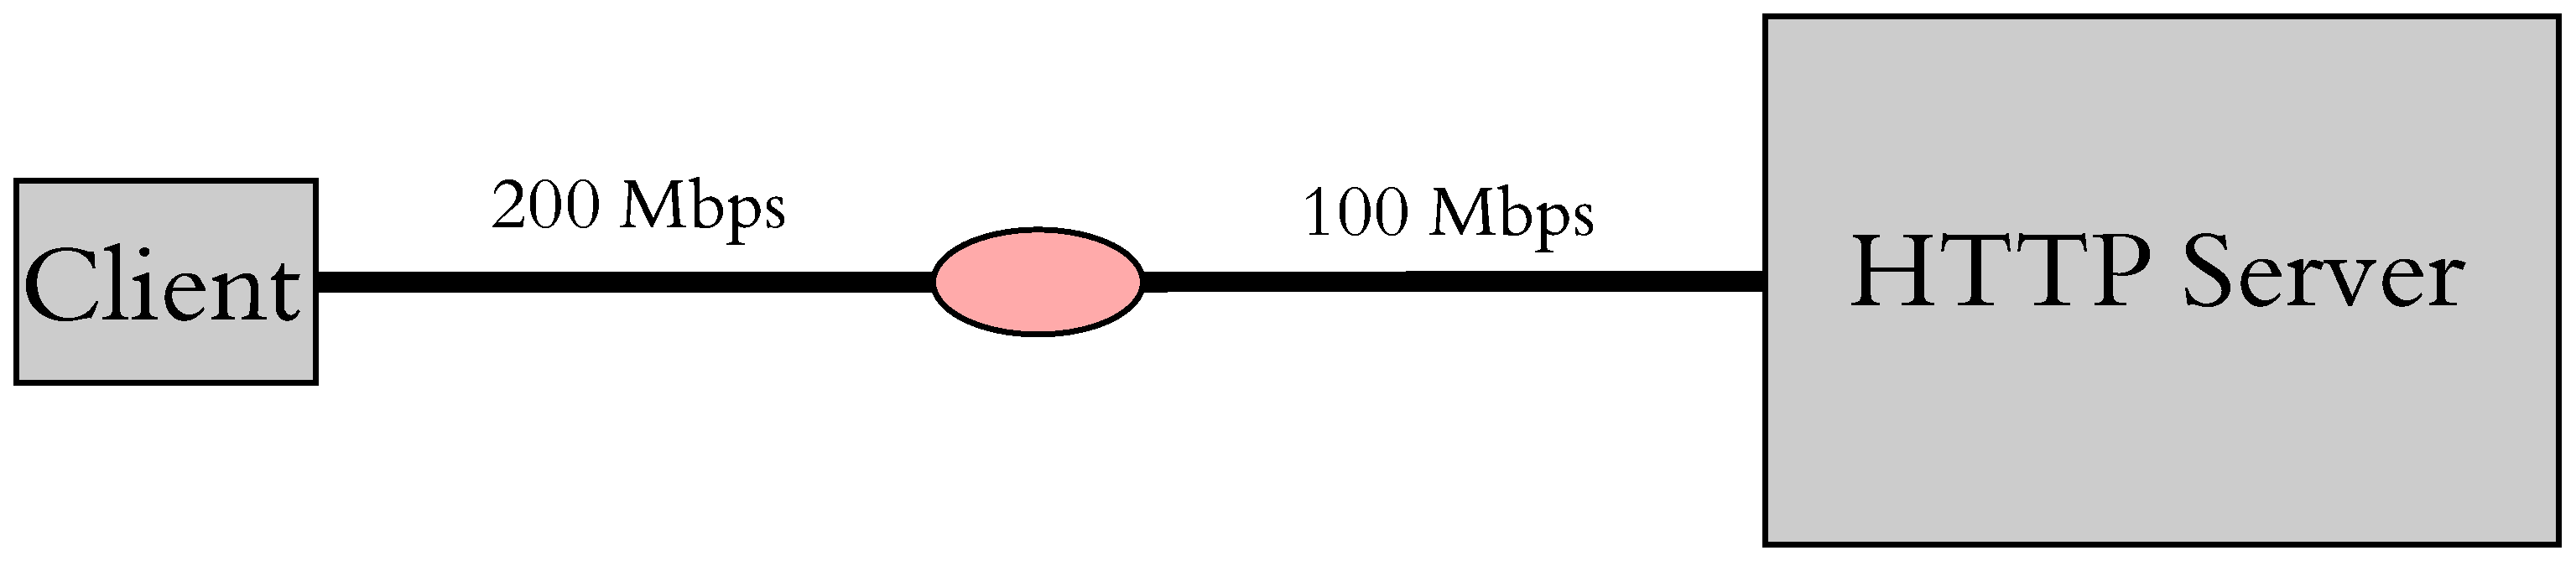
\includegraphics[width=120mm]{Q1.eps}
%\begin{tikzpicture}
%\filldraw[fill=blue!10!white,draw=blue]
%(-1,-0.5)--(1,-0.5)--(1,0.5)--(-1,0.5)--(-1,-0.5);
%\node at(0,0) {Client};
%\end{tikzpicture}
\end{figure}

نرخ ارسال هر یک از لینک ها، در بالای آنها ذکر شده است. فرض کنید کاربر قصد دارد صفحه‌ی وبی را که شامل آدرس 5 فایل 1 مگابایتی می‌باشد، به همراه آن 5 فایل دانلود کند. اگر تاخیر پردازش روتر برای هر یک از 5 فایل 1 مگابایتی برابر 10 میلی ثانیه باشد، نرخ موثر دانلود صفحه‌ی وب به همراه 5 فایل داخل آن چقدر است اگر

الف) اتصال از نوع \lr{non-persistent} باشد؟

ب) اتصال از نوع \lr{persistent} باشد؟

(مقدار RTT برابر 5 میلی ثانیه است. سایر تاخیرها را صفر بگیرید. حجم صفحه‌ی وب به تنهایی ناچیز است.)

(برای محاسبه‌ی نرخ موثر دانلود، کل حجم دانلود شده توسط کاربر را تقسیم بر کل زمان مصرف شده از ابتدای برقراری ارتباطات TCP تا پایان نمایید.)

\newpage
\Q

5 کاربر توسط لینکی با ظرفیت \lr{3Mbps} به اینترنت دسترسی دارند. هر کاربر، دارای نرخ درخواستی \lr{1Mbps} و احتمال فعال بودن $p=0.6$ است. اگر مجموع ظرفیت اشغال شده توسط کاربران فعال (استفاده کننده از لینک) از ظرفیت لینک بیشتر باشد، دسترسی تمام کاربران فعال به اینترنت قطع می‌شود.

\begin{figure}[h]
\centering
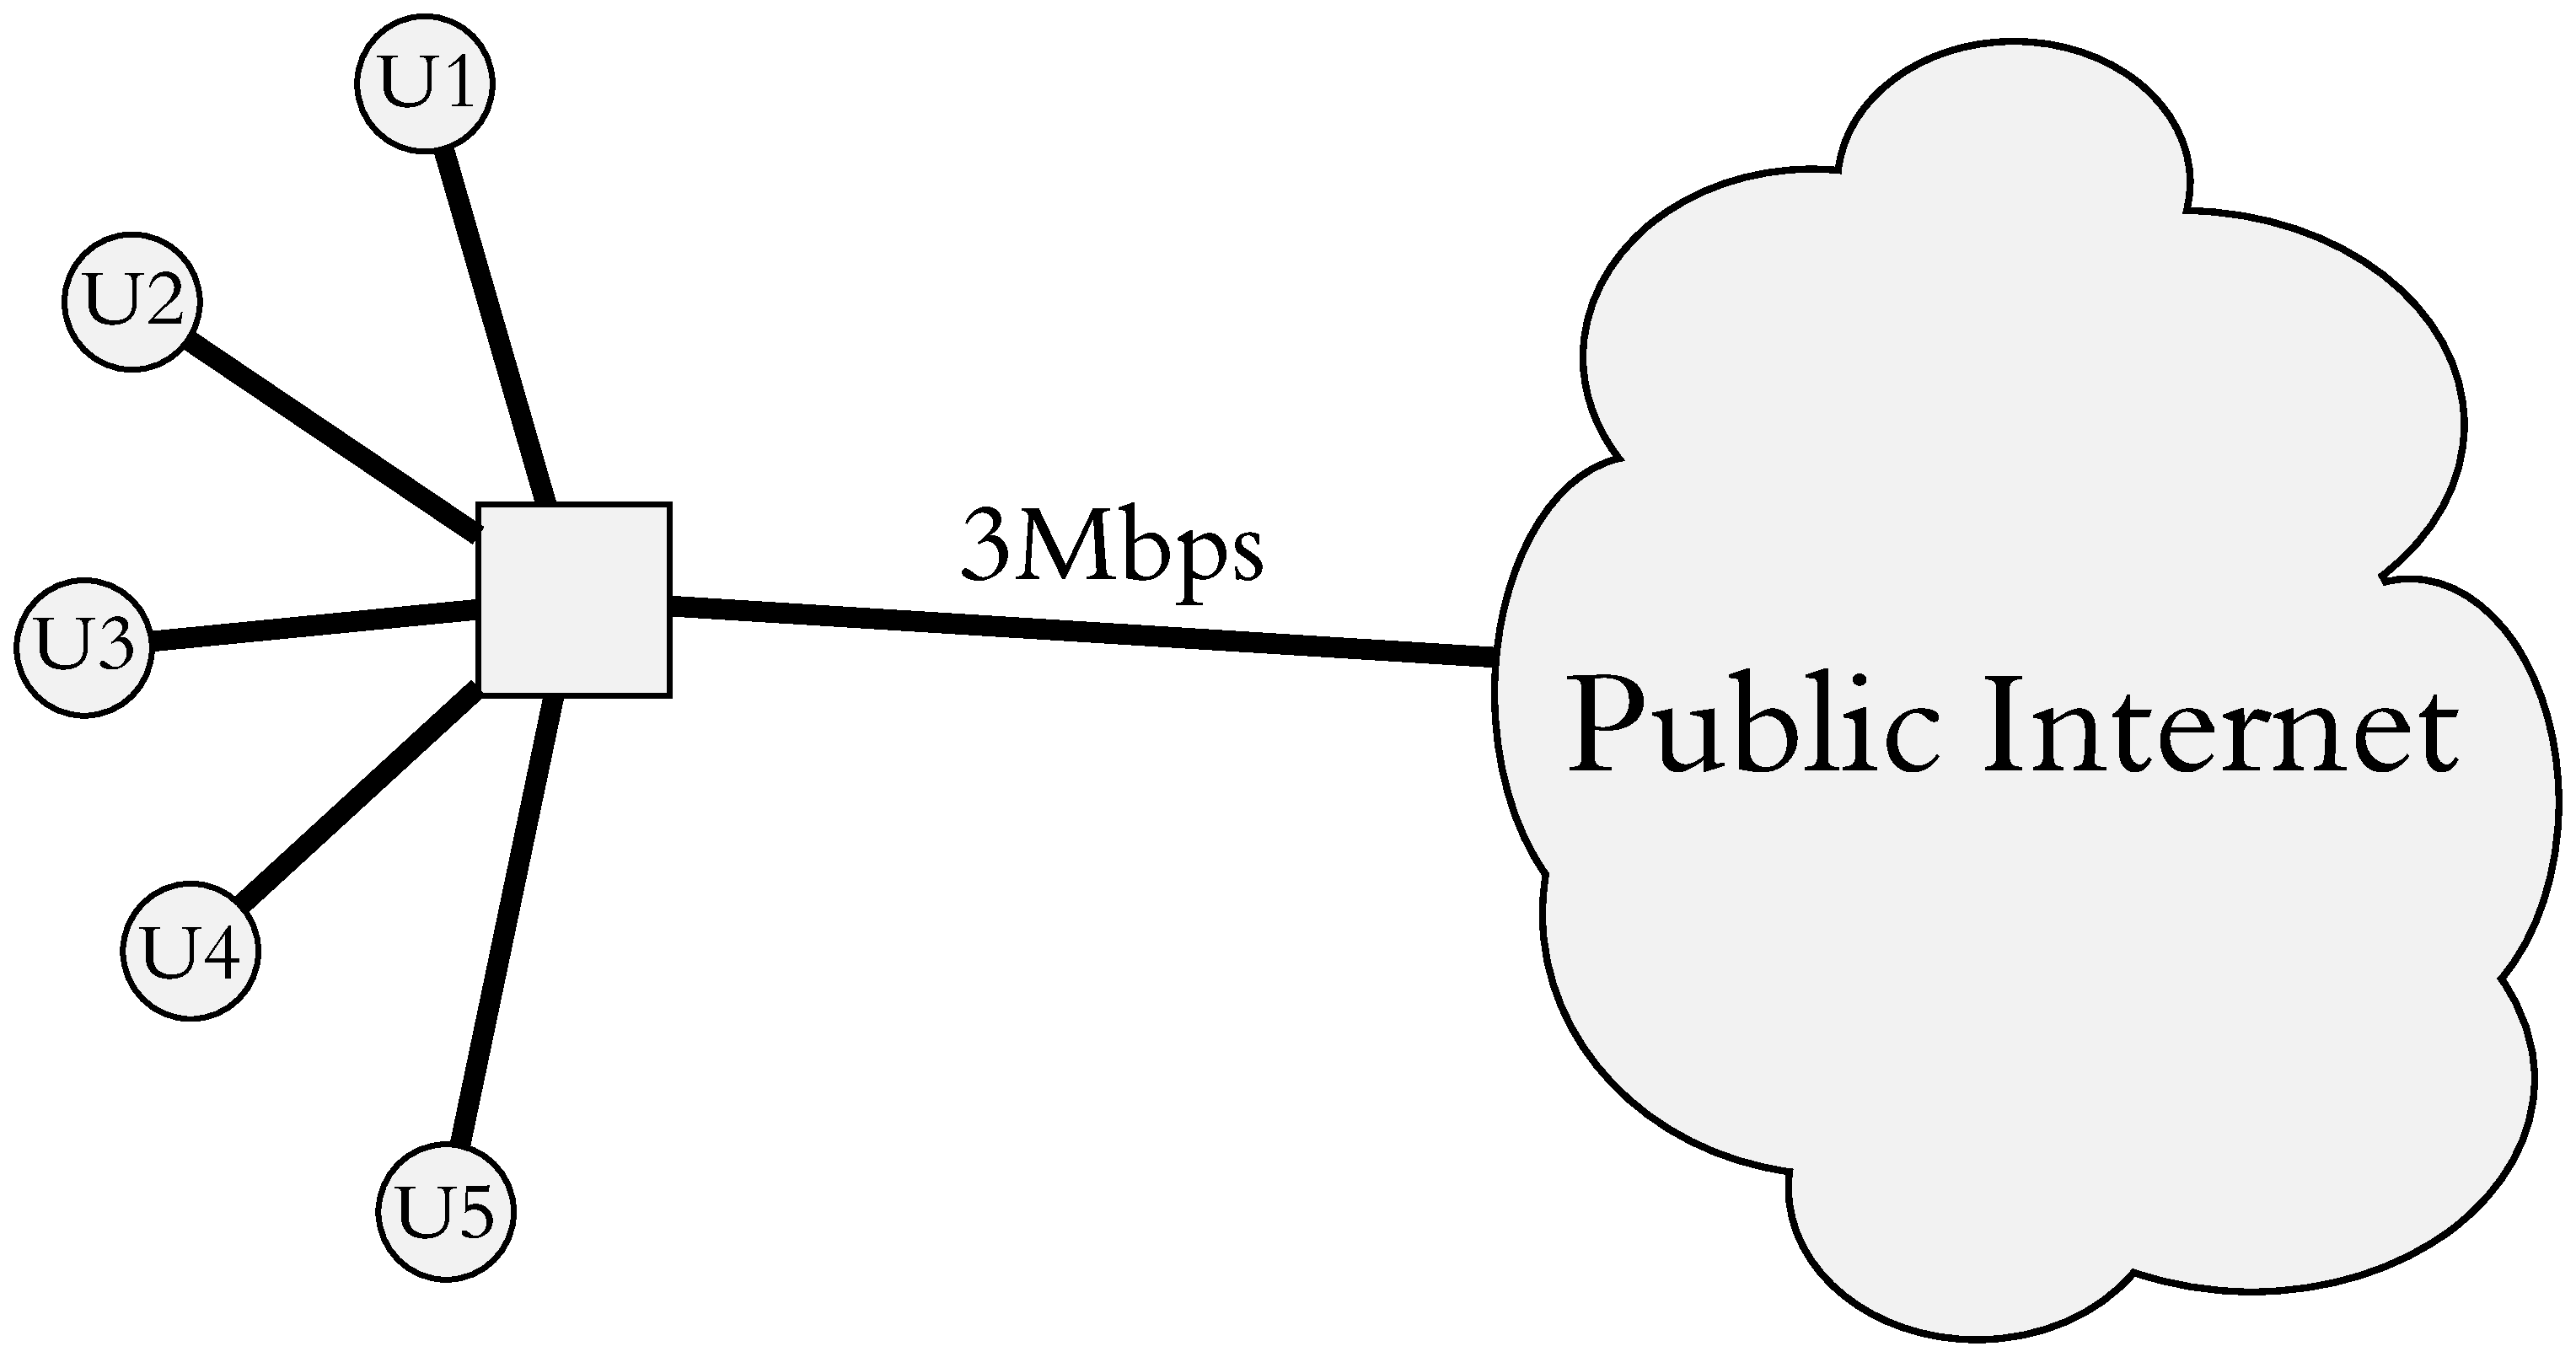
\includegraphics[width=100mm]{Q2_1.eps}
\end{figure}

الف) احتمال آن که کاربران فعال بتوانند از لینک بدون قطعی اتصال استفاده کنند چقدر است؟

ب) اگر کاربران به یک \lr{Web Cache Server} متصل شوند که بتواند 30درصد نیاز (پهنای باند) کاربران را به صورت محلی (\lr{Local}) برآورده کند، احتمال آن که سایر کاربران فعال بتوانند از لینک بدون قطعی اتصال به اینترنت استفاده کنند چقدر است؟

%ب) فرض کنید یک \lr{Web Cache Server} در شبکه‌ی محلی تعبیه شده است
\begin{figure}[h]
\centering
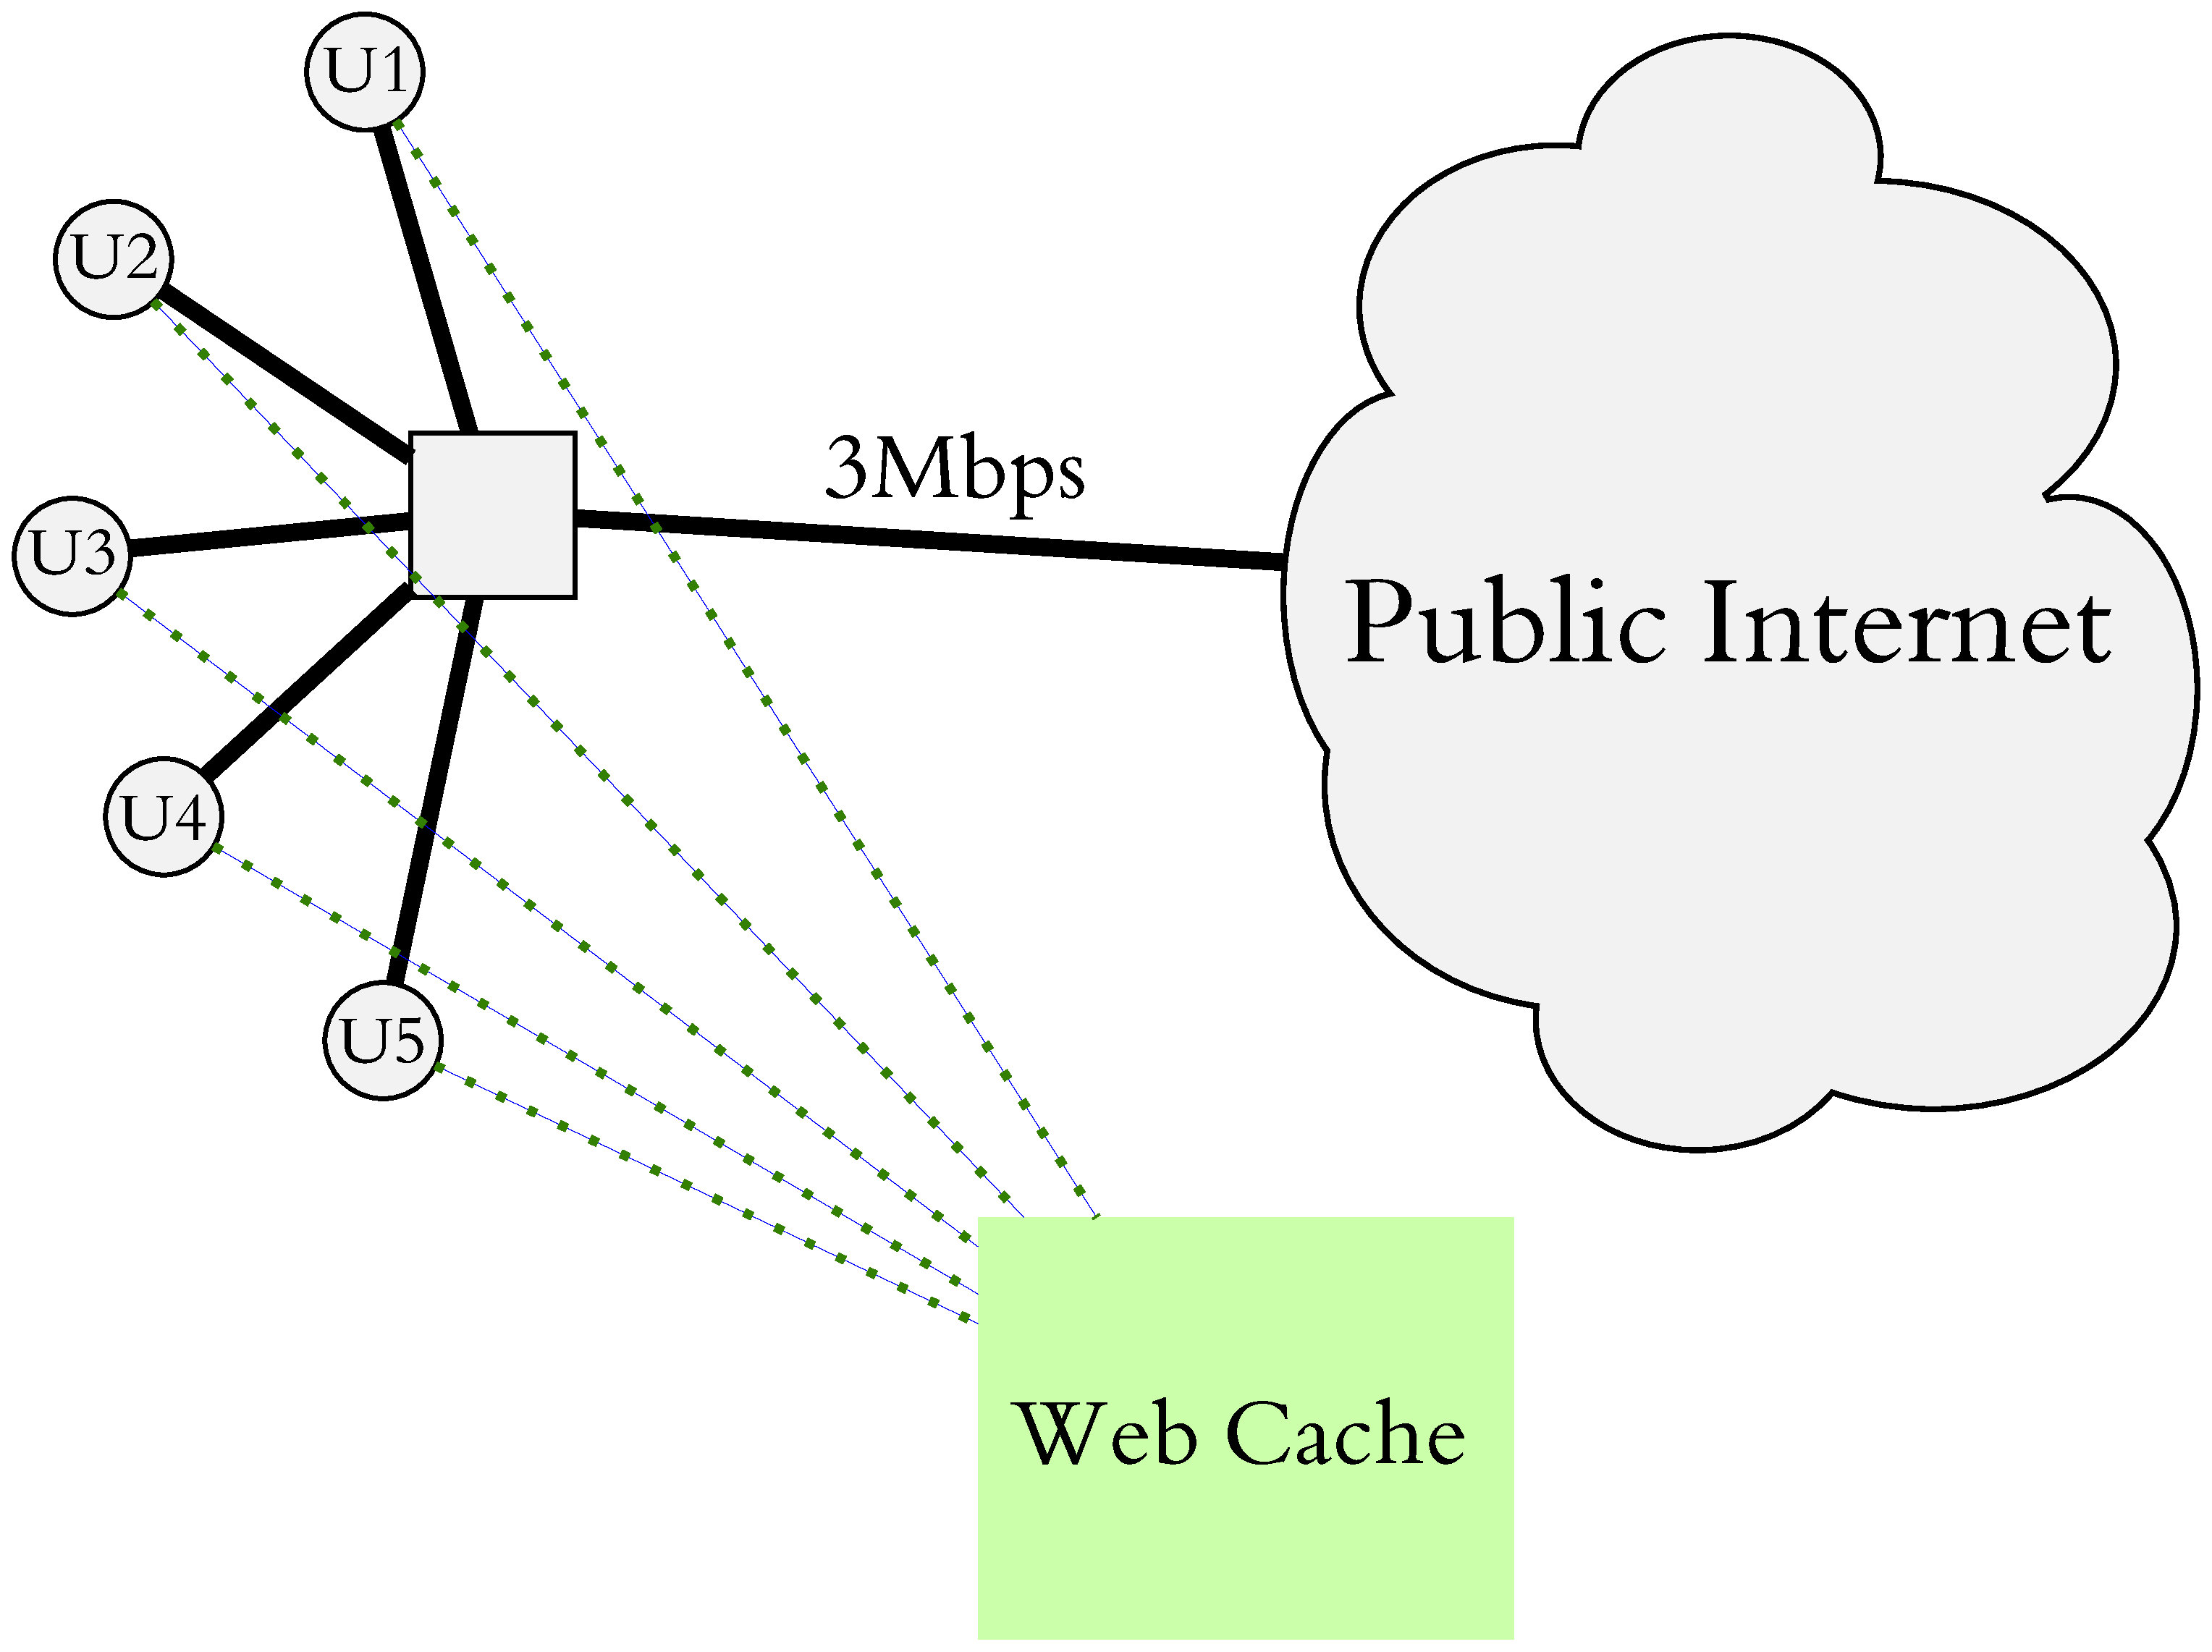
\includegraphics[width=100mm]{Q2_2.eps}
\end{figure}

\newpage
\Q

یک فرستنده و یک گیرنده‌ی \lr{TCP}، توسط یک کانال مخابراتی به هم متصل شده اند. فرستنده از مکانیزم \lr{Selective Repeat} برای ارسال و تشخیص خطای بسته استفاده می‌کند. فرض کنید این کانال با احتمال
$
p_1
$،
هر بسته‌ی ارسالی از فرستنده به گیرنده و با احتمال 
$
p_2
$،
هر \lr{ACK} از گیرنده به فرستنده را از بین می‌برد. این فرستنده باید به طور متوسط هر بسته را چند بار بفرستد تا \lr{ACK} آن را از گیرنده دریافت کند؟

(برای محاسبه‌ی متوسط تعداد دفعات ارسالی تا دریافت موفق \lr{ACK} از سوی گیرنده، باید ابتدا احتمال دریافت موفق \lr{ACK} از سوی گیرنده در $k$ بار ارسال بسته را به ازای $k\in\Bbb N$ محاسبه کرده و سپس، امید ریاضی احتمال های فوق را به دست آورید.)

($\sum_{k=1}^\infty ka^k=\frac{a}{(1-a)^2}\quad , \quad |a|<1$)

\newpage
\Q

یک فرستنده و یک گیرنده‌ی \lr{TCP} ، از مکانیزم \lr{TCP Congestion Control} برای کنترل نرخ ارسال فرستنده به گیرنده بهره می‌برند. نمودار طول پنجره‌ی فرستنده (\lr{cwnd}) بر حسب دور ارسال به صورت زیر است:
\begin{figure}[h]
\centering
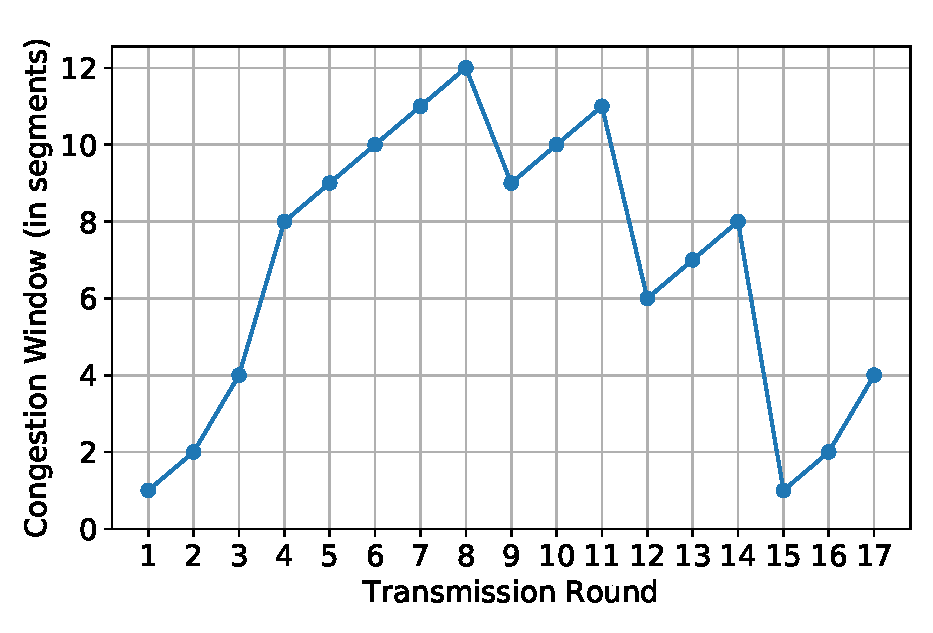
\includegraphics[width=120mm]{Q4.eps}
\end{figure}

الف) فرستنده از کدام یک از مکانیزم های \lr{Reno} یا \lr{Tahoe} استفاده کرده است؟ چرا؟

ب) فرستنده در دور ارسال 8، از چه حالت به چه حالتی رفته است؟

ب) فرستنده در دور ارسال 11، از چه حالت به چه حالتی رفته است؟

ت) فرستنده در دور ارسال 14، چه خطایی (\lr{Timeout} یا \lr{3-duplicate ACKs}) را آشکار می‌کند؟

ث) در دور ارسال 15، مقدار \lr{ssthresh} چقدر است؟

ج) در کدام دور ارسال از 1 تا 17، \lr{ssthresh} بیشترین مقدار خود را می‌گیرد؟

(فرض کنید مقدار اولیه‌ی \lr{ssthresh} برابر 8 است.)
\end{document}